\section{Evaluation}

% Slide 8: Experimental Validation
\begin{frame}{Experimental Validation}{Power Balancing Performance under Volatility}
  \begin{columns}[T]
    \begin{column}{0.48\textwidth}
      \textbf{Simulation Setup}:
      \begin{itemize}
        \item 10-node microgrid simulation.
        \item Fictional solar generation profiles from Nimbus database.
        \item Real-time pricing fluctuations.
      \end{itemize}
      \vspace{0.3cm}
      \textbf{Key Observations}:
      \begin{itemize}
        \item Proposed Synapse method tracks optimal Centralized MPC closely.
        \item Significantly outperforms traditional Rule-Based heuristics.
      \end{itemize}
    \end{column}
    
    \begin{column}{0.48\textwidth}
      \centering
      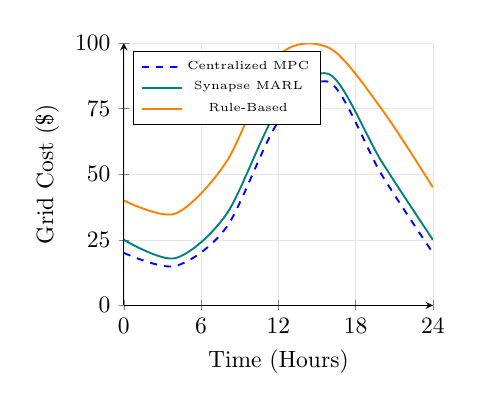
\begin{tikzpicture}[scale=0.85]
        \begin{axis}[
          width=6.2cm,
          height=5.5cm,
          xlabel={Time (Hours)},
          ylabel={Grid Cost (\$)},
          xmin=0, xmax=24,
          ymin=0, ymax=100,
          xtick={0,6,12,18,24},
          ytick={0,25,50,75,100},
          legend pos=north west,
          legend style={font=\tiny},
          grid=both,
          grid style={line width=.1pt, draw=gray!10},
          major grid style={line width=.2pt, draw=gray!20},
          axis lines=left
        ]
        % MPC Baseline
        \addplot[smooth, blue, dashed, thick] coordinates {
          (0,20) (4,15) (8,30) (12,70) (16,85) (20,50) (24,20)
        };
        \addlegendentry{Centralized MPC}
        
        % Proposed MARL
        \addplot[smooth, teal, thick] coordinates {
          (0,25) (4,18) (8,35) (12,75) (16,88) (20,55) (24,25)
        };
        \addlegendentry{Synapse MARL}
        
        % Rule-Based
        \addplot[smooth, orange, thick] coordinates {
          (0,40) (4,35) (8,55) (12,95) (16,98) (20,75) (24,45)
        };
        \addlegendentry{Rule-Based}
        \end{axis}
      \end{tikzpicture}
    \end{column}
  \end{columns}
\end{frame}

% Slide 9: Performance Metrics Table
\begin{frame}{Performance Metrics}{Quantitative System Evaluation}
  We evaluate the algorithms across 1,000 independent runs. Cost and carbon metrics are normalized.
  \vspace{0.4cm}
  
  \centering
  \resizebox{\textwidth}{!}{%
    \begin{tabular}{lcccc}
      \toprule
      \textbf{Optimization Method} & \textbf{Time to Converge (s)} & \textbf{Daily Cost (\$)} & \textbf{Carbon (kg)} & \textbf{Feasibility (\%)} \\
      \midrule
      \rowcolor{VertexBlue!10}
      Centralized MPC & 124.50 & 42.10 & 120.4 & 100.0 \\
      Rule-Based Heuristic & 0.05 & 68.30 & 185.2 & 92.4 \\
      Decentralized Q-Learning & 1.20 & 55.40 & 152.0 & 94.8 \\
      \textbf{Synapse MARL (Ours)} & \textbf{0.45} & \textbf{44.80} & \textbf{128.6} & \textbf{99.8} \\
      \bottomrule
    \end{tabular}%
  }
\end{frame}

% Slide 10: Block Types Comparison
\begin{frame}{System Capabilities}{Standard Rochester Block Implementations}
  The Rochester theme provides distinctive colored blocks to structure different types of content:
  \vspace{0.2cm}
  
  \begin{block}{Standard Block: Core System Features}
    Used for general statements, definitions, or standard descriptions of algorithm components.
  \end{block}
  
  \begin{alertblock}{Alert Block: Critical Operational Limits}
    Used to highlight critical constraints, safety violation thresholds, or convergence failure states.
  \end{alertblock}
  
  \begin{exampleblock}{Example Block: Localized Node Configuration}
    Used for case examples, specific physical parameters, or demonstration scenarios.
  \end{exampleblock}
\end{frame}

% Slide 11: Case Study
\begin{frame}{Case Study: Meridian Pilot}{Field Implementation and Performance}
  To evaluate performance in production, we deployed the Synapse system at the Meridian Microgrid facility.
  \vspace{0.4cm}
  
  \begin{columns}[T]
    \begin{column}{0.48\textwidth}
      \begin{tcolorbox}[
        colback=VertexBlue!5,
        colframe=VertexBlue,
        title=Deployment Profile,
        fonttitle=\bfseries\small,
        arc=2mm,
        left=2mm, right=2mm, top=2mm, bottom=2mm
      ]
        \small
        \begin{itemize}
          \item \textbf{Location}: Apex Industrial Zone
          \item \textbf{Capacity}: 2.4 MW peak load
          \item \textbf{Renewables}: 1.2 MW solar PV, 800 kW battery storage
          \item \textbf{Duration}: 90-day trial period
        \end{itemize}
      \end{tcolorbox}
    \end{column}
    
    \begin{column}{0.48\textwidth}
      \begin{tcolorbox}[
        colback=VertexTeal!5,
        colframe=VertexTeal,
        title=Key Outcomes,
        fonttitle=\bfseries\small,
        arc=2mm,
        left=2mm, right=2mm, top=2mm, bottom=2mm
      ]
        \small
        \begin{itemize}
          \item \textbf{Cost Savings}: 22.4\% reduction in peak demand charges
          \item \textbf{Stability}: Zero power outages during high volatility
          \item \textbf{Efficiency}: 98.6\% local solar consumption rate
        \end{itemize}
      \end{tcolorbox}
    \end{column}
  \end{columns}
\end{frame}
